\documentclass{beamer}

\mode<presentation> {

\usetheme{default}
\usecolortheme{default}

%\setbeamertemplate{footline} % To remove the footer line in all slides uncomment this line
%\setbeamertemplate{footline}[page number] % To replace the footer line in all slides with a simple slide count uncomment this line
%\setbeamertemplate{navigation symbols}{} % To remove the navigation symbols from the bottom of all slides uncomment this line
}

\usepackage{graphicx} % Allows including images
\usepackage{booktabs} % Allows the use of \toprule, \midrule and \bottomrule in tables
\setbeamertemplate{caption}{\insertcaption} 
\setbeamertemplate{caption label separator}{}
\setbeamerfont{frametitle}{size=\Large}

\newenvironment{graytext}{\color{gray}}{\ignorespacesafterend}

%----------------------------------------------------------------------------------------
%	TITLE PAGE
%----------------------------------------------------------------------------------------

\title[Twe data summer 2014]{Twe data summer 2014} % The short title appears at the bottom of every slide, the full title is only on the title page

\author{Layne J. Vashro} % Your name
\institute[Utah] % Your institution as it will appear on the bottom of every slide, may be shorthand to save space
{
University of Utah \\ % Your institution for the title page
\medskip
\textit{Layne.Vashro@anthro.utah.edu} % Your email address
}
\date{\today} % Date, can be changed to a custom date

\begin{document}

\begin{frame}
\titlepage % Print the title page as the first slide
\end{frame}

%------------------------------------------------

%\begin{frame}<beamer>{Table of Contents}
%\tableofcontents[hidesubsections]
%\end{frame}

%------------------------------------------------
%------------------------------------------------

\section{Introduction}

%------------------------------------------------
%------------------------------------------------

\begin{frame}

\frametitle{Tasks}

Cognition: 3DMR, Corsi, Perspective-taking \\
\vspace{0.75cm}
Anxiety: Harm-avoidance, Spatial anxiety \\
\vspace{0.75cm}
Navigation: Pointing task \\
\vspace{0.75cm}
Mobility: Trackers (daily), Interviews (annual, lifetime)

\end{frame}

%------------------------------------------------

\begin{frame}
\frametitle{Who leaves home and when?}
\begin{columns}[c] % The "c" option specifies centered vertical alignment while the "t" option is used for top vertical alignment

\column{.45\textwidth} % Left column and width

Household exogamy \\
\vspace{0.25cm}
Postmarital residence \\
\vspace{0.25cm}
Dispersal \\
\vspace{0.25cm}
Explaining variation
	\begin{itemize}
		\item cross-cultural vs. local
	\end{itemize}

\column{.5\textwidth} % Right column and width
\includegraphics[width= 1\textwidth]{twe_couple}

\end{columns}
\end{frame}

%------------------------------------------------

\begin{frame}
\frametitle{Flexible Residence of Foragers}

Modal forager residence pattern is ``flexible'' (Alvarez 2004, Marlowe 2004) \\
\vspace{0.75cm}
Even when listed as ``strict'' residence, may not be accurate (Hill et al. 2011) \\
\vspace{0.75cm}
Without strict residence, group-level explanation don't help

\end{frame}

%------------------------------------------------

%\begin{frame}
%\frametitle{Patterning of the flexibility?}
%\begin{table}
%\caption{Early and Late residence across 35 forager societies in the SCCS.  Table adapted from Marlowe (2004)}
%\begin{tabular}{c c c}
%\toprule
%\textbf{Residence} & \textbf{Early Transfer} & \textbf{Late Transfer}\\
%\midrule
%Virilocal & 34.3\% & \textbf{57.1\%}\\
%Multilocal & 17.1\% & 20\%\\
%Uxorilocal & \textbf{48.6\%} & 22.9\%\\
%\bottomrule
%\end{tabular}
%\caption{Uxorilocality more common early.  Virilocality more common late.}
%\end{table}
%\end{frame}

%------------------------------------------------

\begin{frame}
\frametitle{Patterning of the flexibility}

\begin{columns}
\begin{column}{.5\textwidth}
Delayed female dispersal:
	\begin{itemize}
		\item Matri-patrilocality (SCCS)
		\item Hadza (Blurton Jones 2005)
		\item Ache and !Kung (Hill et al. 2011)
		\item Twe
	\end{itemize}
\vspace{0.25cm}
How can this pattern be explained? \\
	\begin{itemize} 
		\item Women seeking childcare assistance
	\end{itemize}
\end{column}

\begin{column}{.5\textwidth}
\includegraphics[width= 1\textwidth]{dispersal}\\
\end{column}
\end{columns}

\end{frame}

%------------------------------------------------

\begin{frame}
\frametitle{Who cares?}

\begin{columns}
\begin{column}{.5\textwidth}
\textbf{Key features:}
\begin{itemize}
\item Female
\item Matrilateral kin \\
(Natal camp)
\item Non-fertile \\
(Grandma!)
\end{itemize}
Grandma and residence
\end{column}

\begin{column}{.5\textwidth}
\includegraphics[width= 1\textwidth]{grannycare}\\
\end{column}
\end{columns}

\end{frame}

%------------------------------------------------

\begin{frame}
\frametitle{Who cares?}

\begin{columns}
\begin{column}{.5\textwidth}
\textbf{Babysitters:}
\begin{itemize}
\item Not available early in career
\item Ages $6 +$
\item Direct care
\item Positive effects \\
(fertility, survival, leisure)
\item Tied to mom rather than natal camp
\end{itemize}
\end{column}

\begin{column}{.5\textwidth}
\begin{figure}
\includegraphics[width= 1\textwidth]{kid_hlprs2}
\end{figure}
\end{column}
\end{columns}

\end{frame}

%------------------------------------------------

\begin{frame}
\frametitle{Who cares? Among the Twe}
\begin{table}
\begin{tabular}{l c c c}
\toprule
\textbf{Relationship} & \textbf{Holder} & \textbf{Available} & \textbf{Percentage}\\ 
\midrule
%Mother & 292 & 398 & 73\%\\
Older sister & 15 & 80 & 18.8\%\\
Mat. Grandma & 7 & 51 & 13.7\%\\
Mat. Cousin & 8 & 90 & 8.9\%\\
Father & 8 & 124 & 6.5\%\\
Pat. Aunt & 1 & 16 & 6.2\%\\
Mat. Aunt & 10 & 320 & 3.1\%\\
\bottomrule
\end{tabular}
\caption{See Kramer (2010) for cross-cultural review}
\end{table}
\end{frame}

%------------------------------------------------

\begin{frame}
\frametitle{Anecdote 1}
\begin{figure}
\includegraphics[width=0.7\linewidth]{natalcmp_care1}
\end{figure}
\end{frame}

%------------------------------------------------

\begin{frame}
\frametitle{Anecdote 2}
\begin{figure}
\includegraphics[width=0.7\linewidth]{kid_hlprs3}
\end{figure}
\end{frame}

%------------------------------------------------

%\begin{frame}
%\frametitle{Who cares? Direct care cross-culturally}
%\begin{table}
%\begin{tabular}{c c c c c}
%\toprule
%\textbf{Mother} & \textbf{Father} & \textbf{Siblings} & \textbf{Grandmas} & \textbf{Other}\\
%\midrule
%47\% & 5\% & 28\% & 9\% & 18\% \\
%\bottomrule
%\end{tabular}
%\caption{Mean proportions of direct care across 9 populations \cite{Kramer}: Ye'kwana, Aka, Efe, Agta, Maya, Alyawara, Trinidad, %Mardu, Toba}
%\end{table}
%\end{frame}

%------------------------------------------------
%------------------------------------------------

\section{Childcare dynamics model}

%------------------------------------------------
%------------------------------------------------

\begin{frame}

\frametitle{Outline}

\begin{graytext}
Introduction \\
\end{graytext}
\vspace{0.75cm}
Simulation: Childcare dynamics \\
\vspace{0.75cm}
Fieldwork: Empirical test among the Twe

\end{frame}

%------------------------------------------------

\begin{frame}
\frametitle{Simulation design}

\begin{columns}
\begin{column}{.5\textwidth}

Female kin group: \\
\begin{itemize}
\item \emph{Ego} \\
\item \emph{G1 (post-repro mom)} \\
\item \emph{G2 (same-aged sister)} \\
\end{itemize}
\vspace{0.5cm}
Track across 20 years

\end{column}

\begin{column}{.5\textwidth}
\includegraphics[width= .9\textwidth]{kingroup}\\
\end{column}
\end{columns}

\end{frame}

%------------------------------------------------

\begin{frame}
\frametitle{Simulation design}

\begin{columns}
\begin{column}{.5\textwidth}
\textbf{Each year:}
\begin{itemize}
\item G2 and Ego reproduce with 25\% chance \\
\vspace{0.5cm}
\item Age $\uparrow$
\end{itemize}
\end{column}

\begin{column}{.5\textwidth}
\centering
\includegraphics[width= .7\textwidth]{repromdl}\\
\includegraphics[width= .8\textwidth]{agingmdl}
\end{column}

\end{columns}
\end{frame}

%------------------------------------------------

\begin{frame}
\frametitle{Simulation design}

\begin{columns}
\begin{column}{.5\textwidth}
Assign age-based need and care points  \\
\vspace{0.5cm}
Eliminate need with care
\end{column}

\begin{column}{.5\textwidth}
\includegraphics[width= .9\textwidth]{needcare}\\
\end{column}
\end{columns}

\end{frame}

%------------------------------------------------

\begin{frame}
\frametitle{Simulation design}

\begin{columns}
\begin{column}{.5\textwidth}
Carer-caree interactions ranked by: relatedness, need, reserves \\
\vspace{0.5cm}
Track \emph{source} of care \\
\vspace{0.5cm}
Residence dependent vs. independent
\end{column}

\begin{column}{.5\textwidth}
\includegraphics[width= .9\textwidth]{distromdl}\\
\end{column}
\end{columns}

\end{frame}

%------------------------------------------------

\begin{frame}
\frametitle{Shifting source of assistance with age}
\begin{figure}
\includegraphics[width=0.6\linewidth]{breakdown}
\end{figure}
\end{frame}

%------------------------------------------------

\begin{frame}
\frametitle{Shifting source of assistance with age}
\begin{figure}
\includegraphics[width=0.6\linewidth]{overview}
\end{figure}
\end{frame}

%------------------------------------------------

\begin{frame}
\frametitle{Simulation discussion}

Within-offspring care ultimately replaces other sources \\
\vspace{0.5cm}
Care-based incentive never drops below 0 \\
\begin{itemize}
\item Only show that costs of leaving decrease
\end{itemize}
\vspace{0.5cm}
Modifications: \\
\begin{itemize}
\item $\uparrow$ \# of sisters
\item delay need/care transition
\end{itemize}

\end{frame}

%------------------------------------------------
%------------------------------------------------

\section{The Twe}

%------------------------------------------------
%------------------------------------------------

\begin{frame}

\frametitle{Outline}

\begin{graytext}
Introduction \\
\vspace{0.75cm}
Simulation: Childcare dynamics \\
\end{graytext}
\vspace{0.75cm}
Fieldwork: Empirical test among the Twe

\end{frame}

%------------------------------------------------

\begin{frame}
\frametitle{The Twe}
\begin{figure}
\includegraphics[width=0.6\linewidth]{thetwe}
\end{figure}
\end{frame}

%------------------------------------------------

\begin{frame}
\frametitle{Map}
\begin{figure}
\includegraphics[width=0.6\linewidth]{bigmap}
\end{figure}
\end{frame}


%------------------------------------------------

\begin{frame}
\frametitle{Lower Kunene Region}

\begin{columns}
\begin{column}{.49\textwidth}
\begin{figure}
\caption{Wet season}
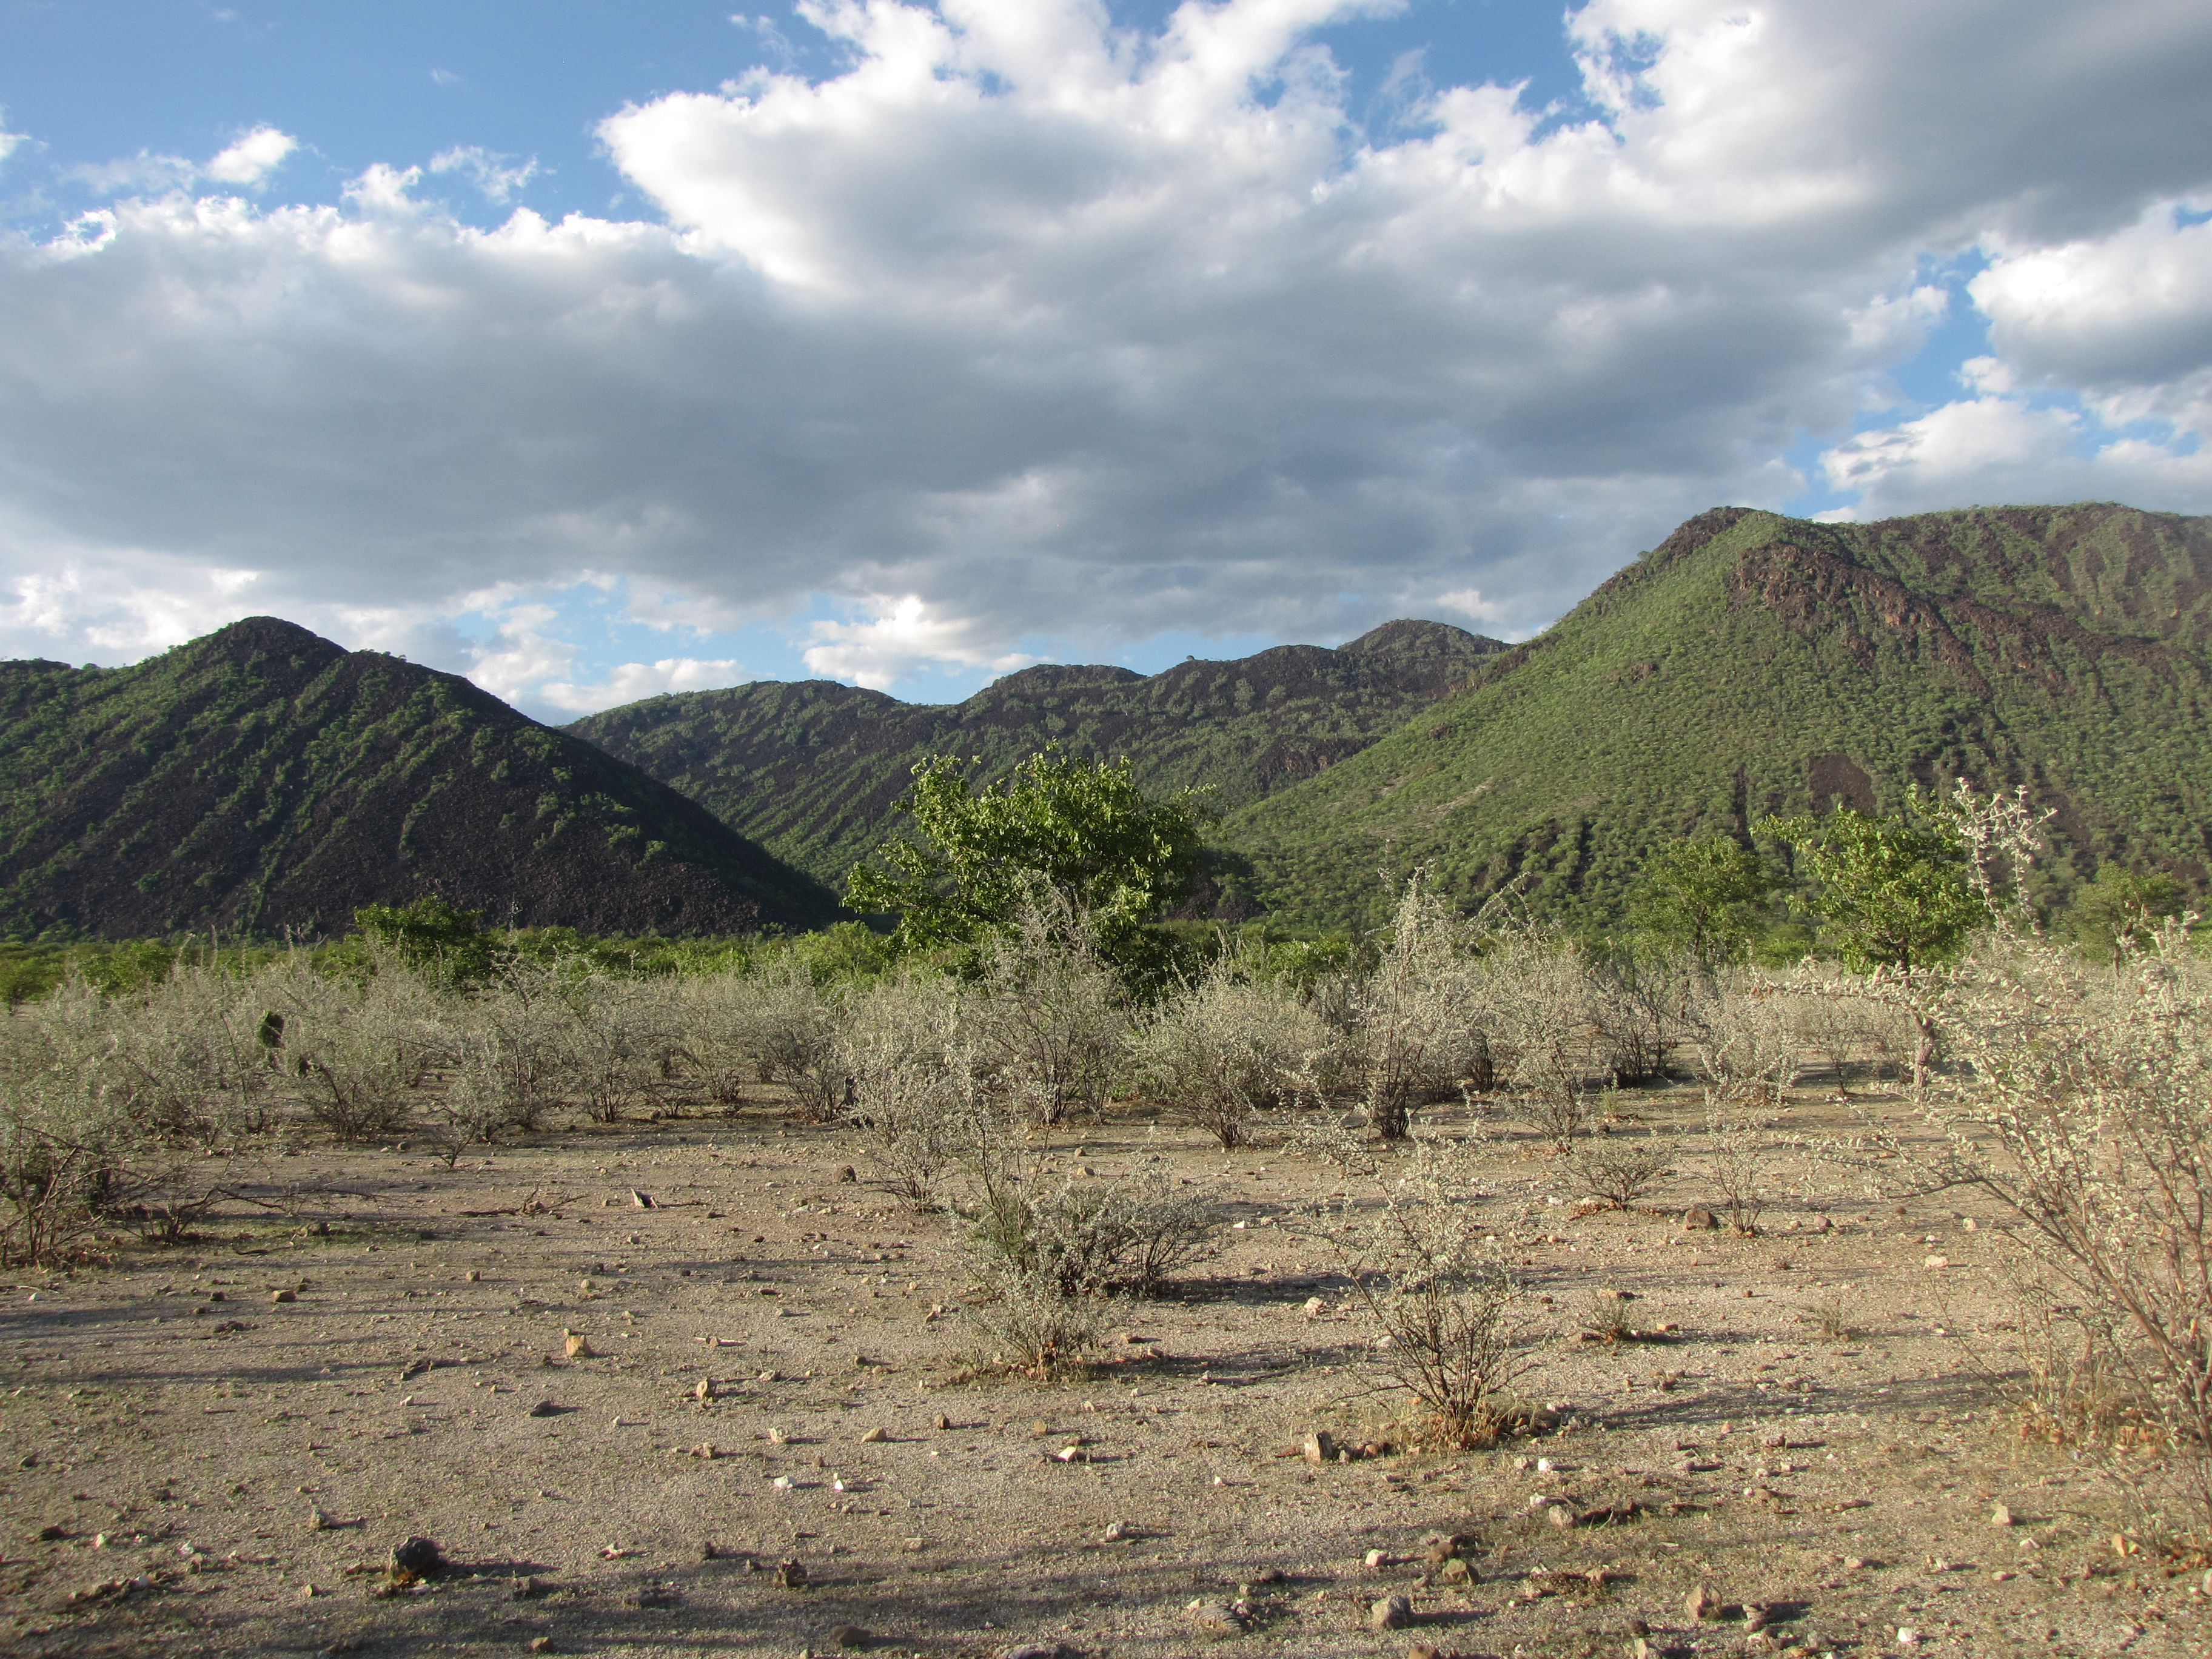
\includegraphics[width= 1\textwidth]{zebramntn}
\end{figure}
\end{column}

\begin{column}{.49\textwidth}
\begin{figure}
\caption{Dry season}
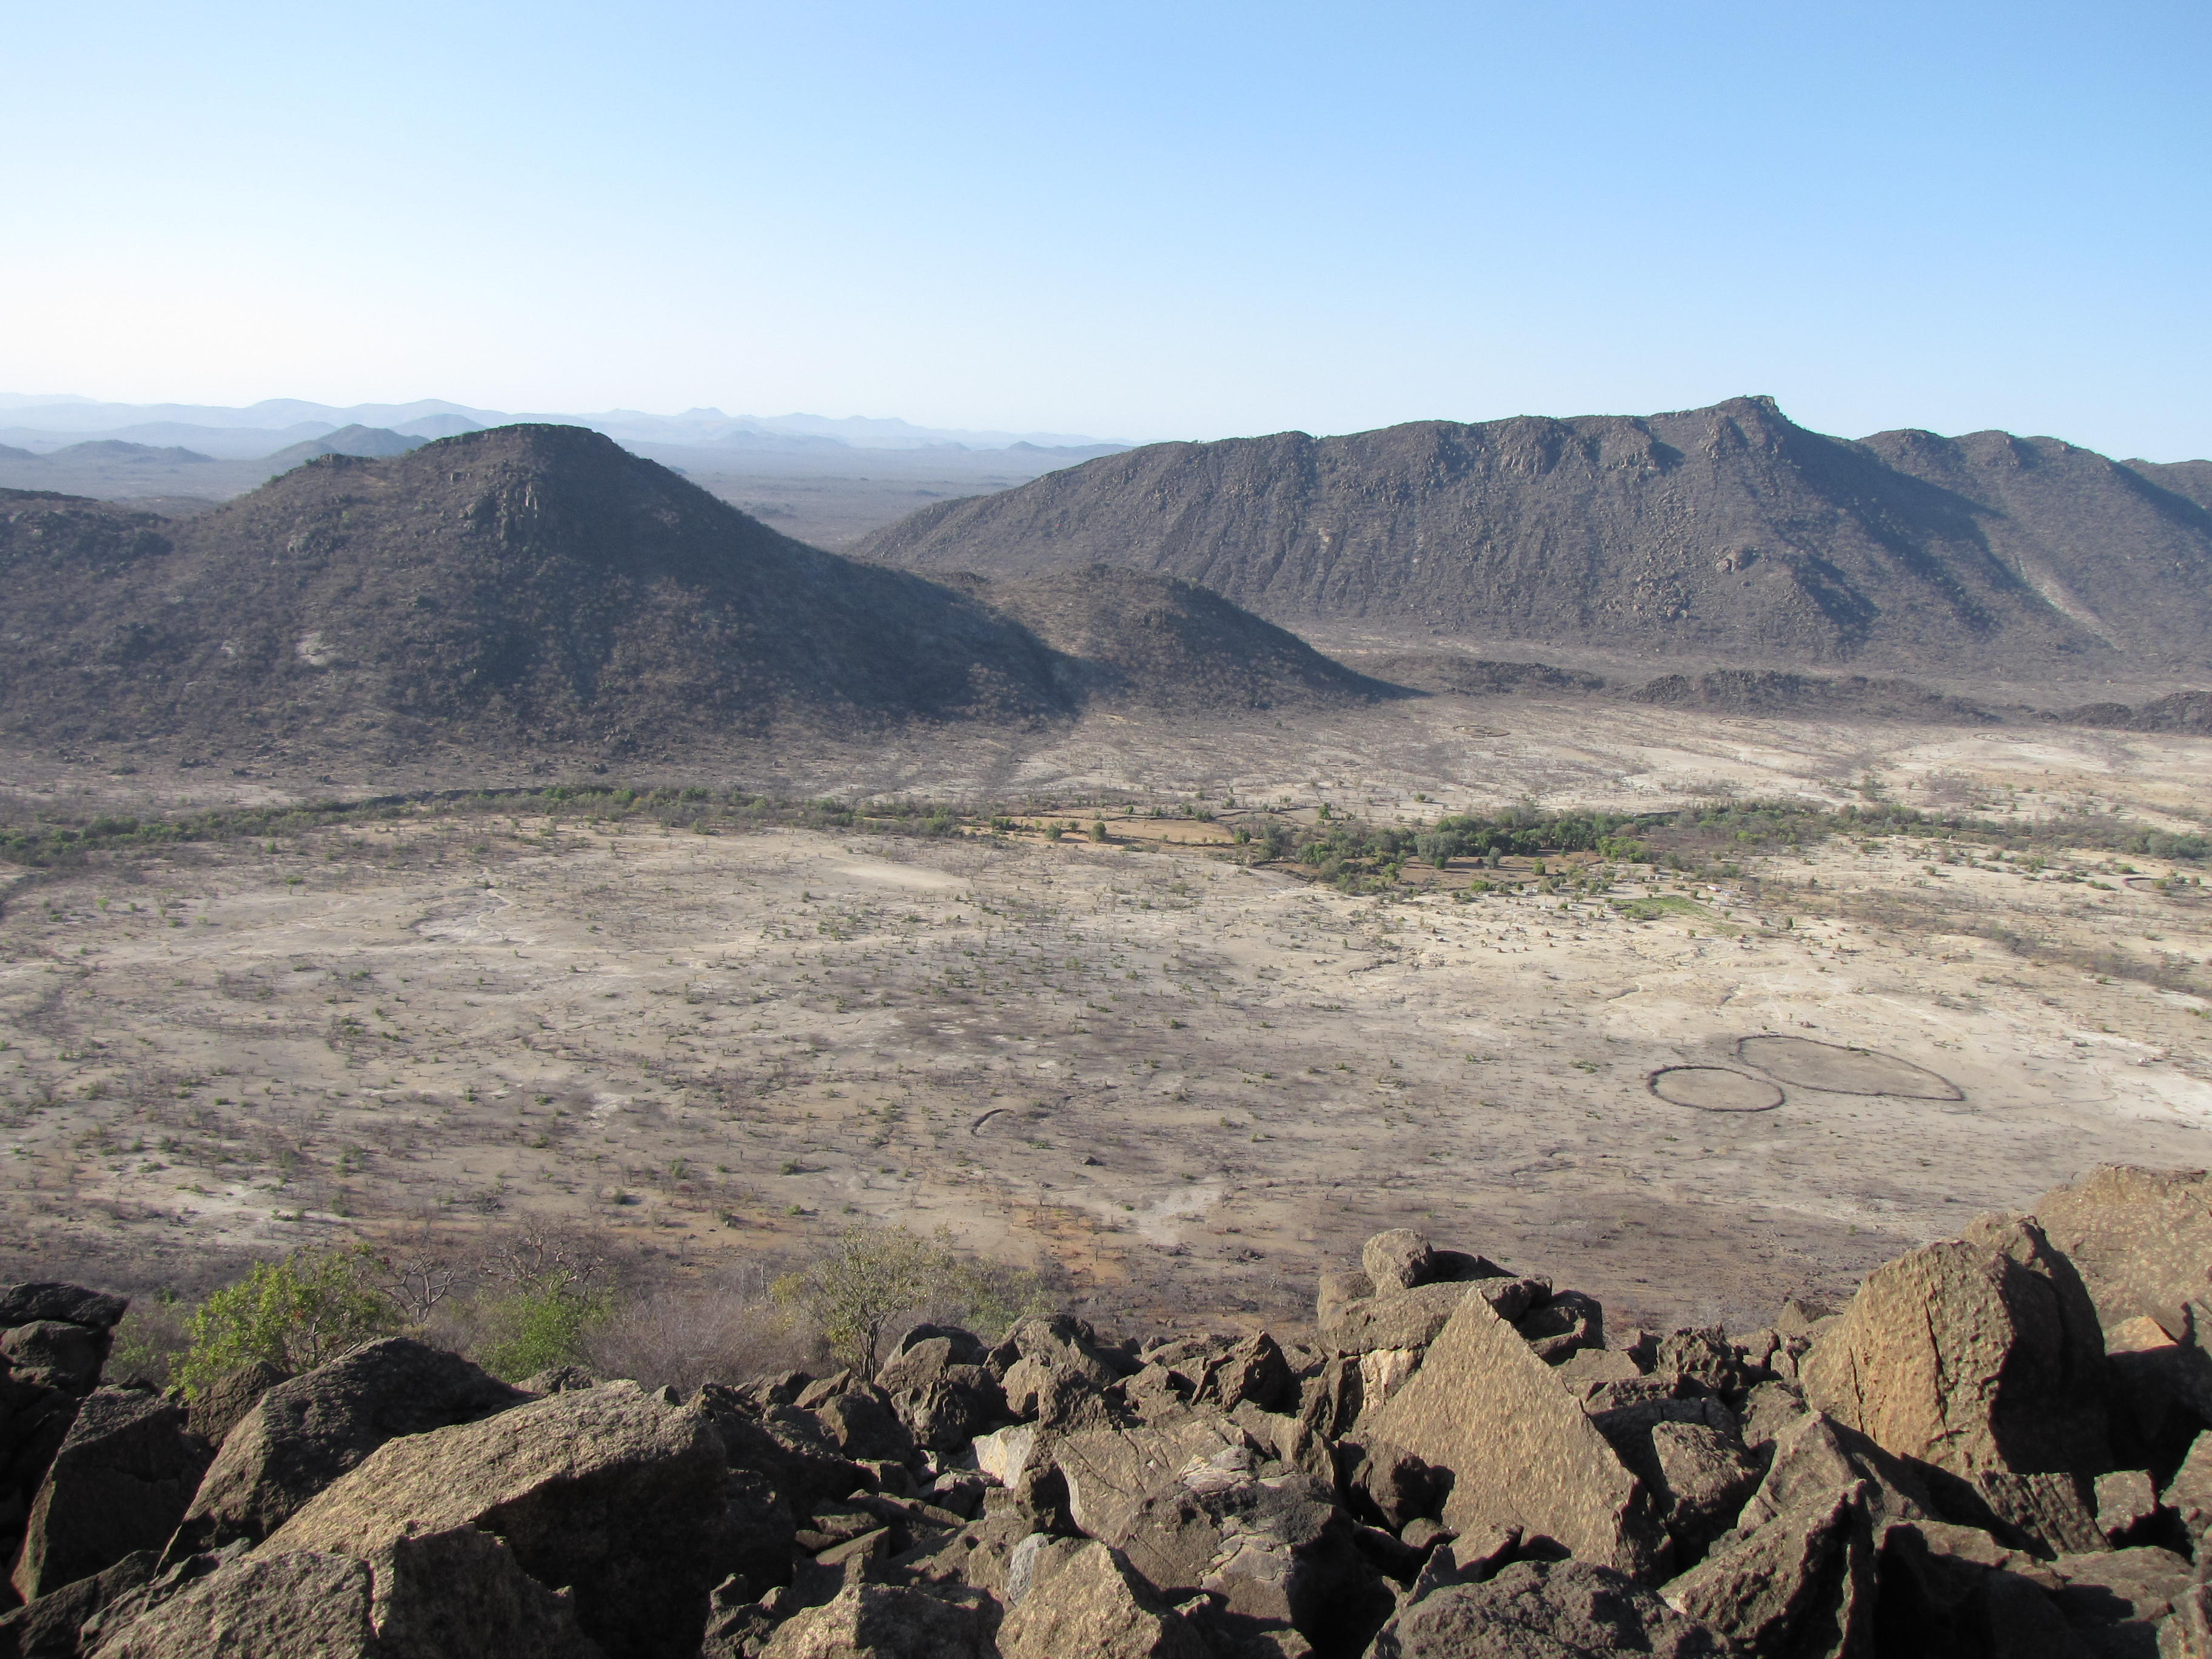
\includegraphics[width= 1\textwidth]{zebramntn2}
\end{figure}
\end{column}
\end{columns}

\end{frame}

%------------------------------------------------

%\begin{frame}
%\frametitle{Bantu neighbors}

%\begin{columns}
%\begin{column}{.5\textwidth}
%\centering
%\includegraphics[width= .8\textwidth]{zemba}\\
%\includegraphics[width= .8\textwidth]{kuvale}
%\end{column}

%\begin{column}{.5\textwidth}
%\centering
%\includegraphics[width= .8\textwidth]{himba}\\
%\includegraphics[width= .8\textwidth]{herero}
%\end{column}
%\end{columns}

%\end{frame}


%------------------------------------------------

%\begin{frame}
%\frametitle{Non-Bantu/Khoisan}
%\begin{figure}
%\includegraphics[width=0.6\linewidth]{nonbantukhoi}
%\end{figure}
%\end{frame}

%------------------------------------------------

\begin{frame}
\frametitle{Subsistence}

\begin{columns}
\begin{column}{.5\textwidth}
\centering
\includegraphics[width= .8\textwidth]{goat}\\
\includegraphics[width= .8\textwidth]{garden_1}
\end{column}

\begin{column}{.5\textwidth}
\centering
\includegraphics[width= .8\textwidth]{ozonjandi}\\
\includegraphics[width= .8\textwidth]{iron_tools}
\end{column}
\end{columns}

\end{frame}

%------------------------------------------------

\begin{frame}
\frametitle{Population distribution}
\begin{figure}
\includegraphics[width=0.8\linewidth]{residence}
\end{figure}
\end{frame}

%------------------------------------------------

\begin{frame}
\frametitle{Delayed female dispersal}
\begin{figure}
\includegraphics[width=0.6\linewidth]{resobs}
\end{figure}
\end{frame}

%------------------------------------------------

\begin{frame}
\frametitle{Fieldwork}

\begin{columns}
\begin{column}{.5\textwidth}
2008 - Present \\
\vspace{0.25cm}
Data collection:
\begin{itemize}
\item Genealogies
\item Reproductive histories 
\item Residence histories 
\item Censuses
\item Behavioral data
\end{itemize}
\end{column}

\begin{column}{.5\textwidth}
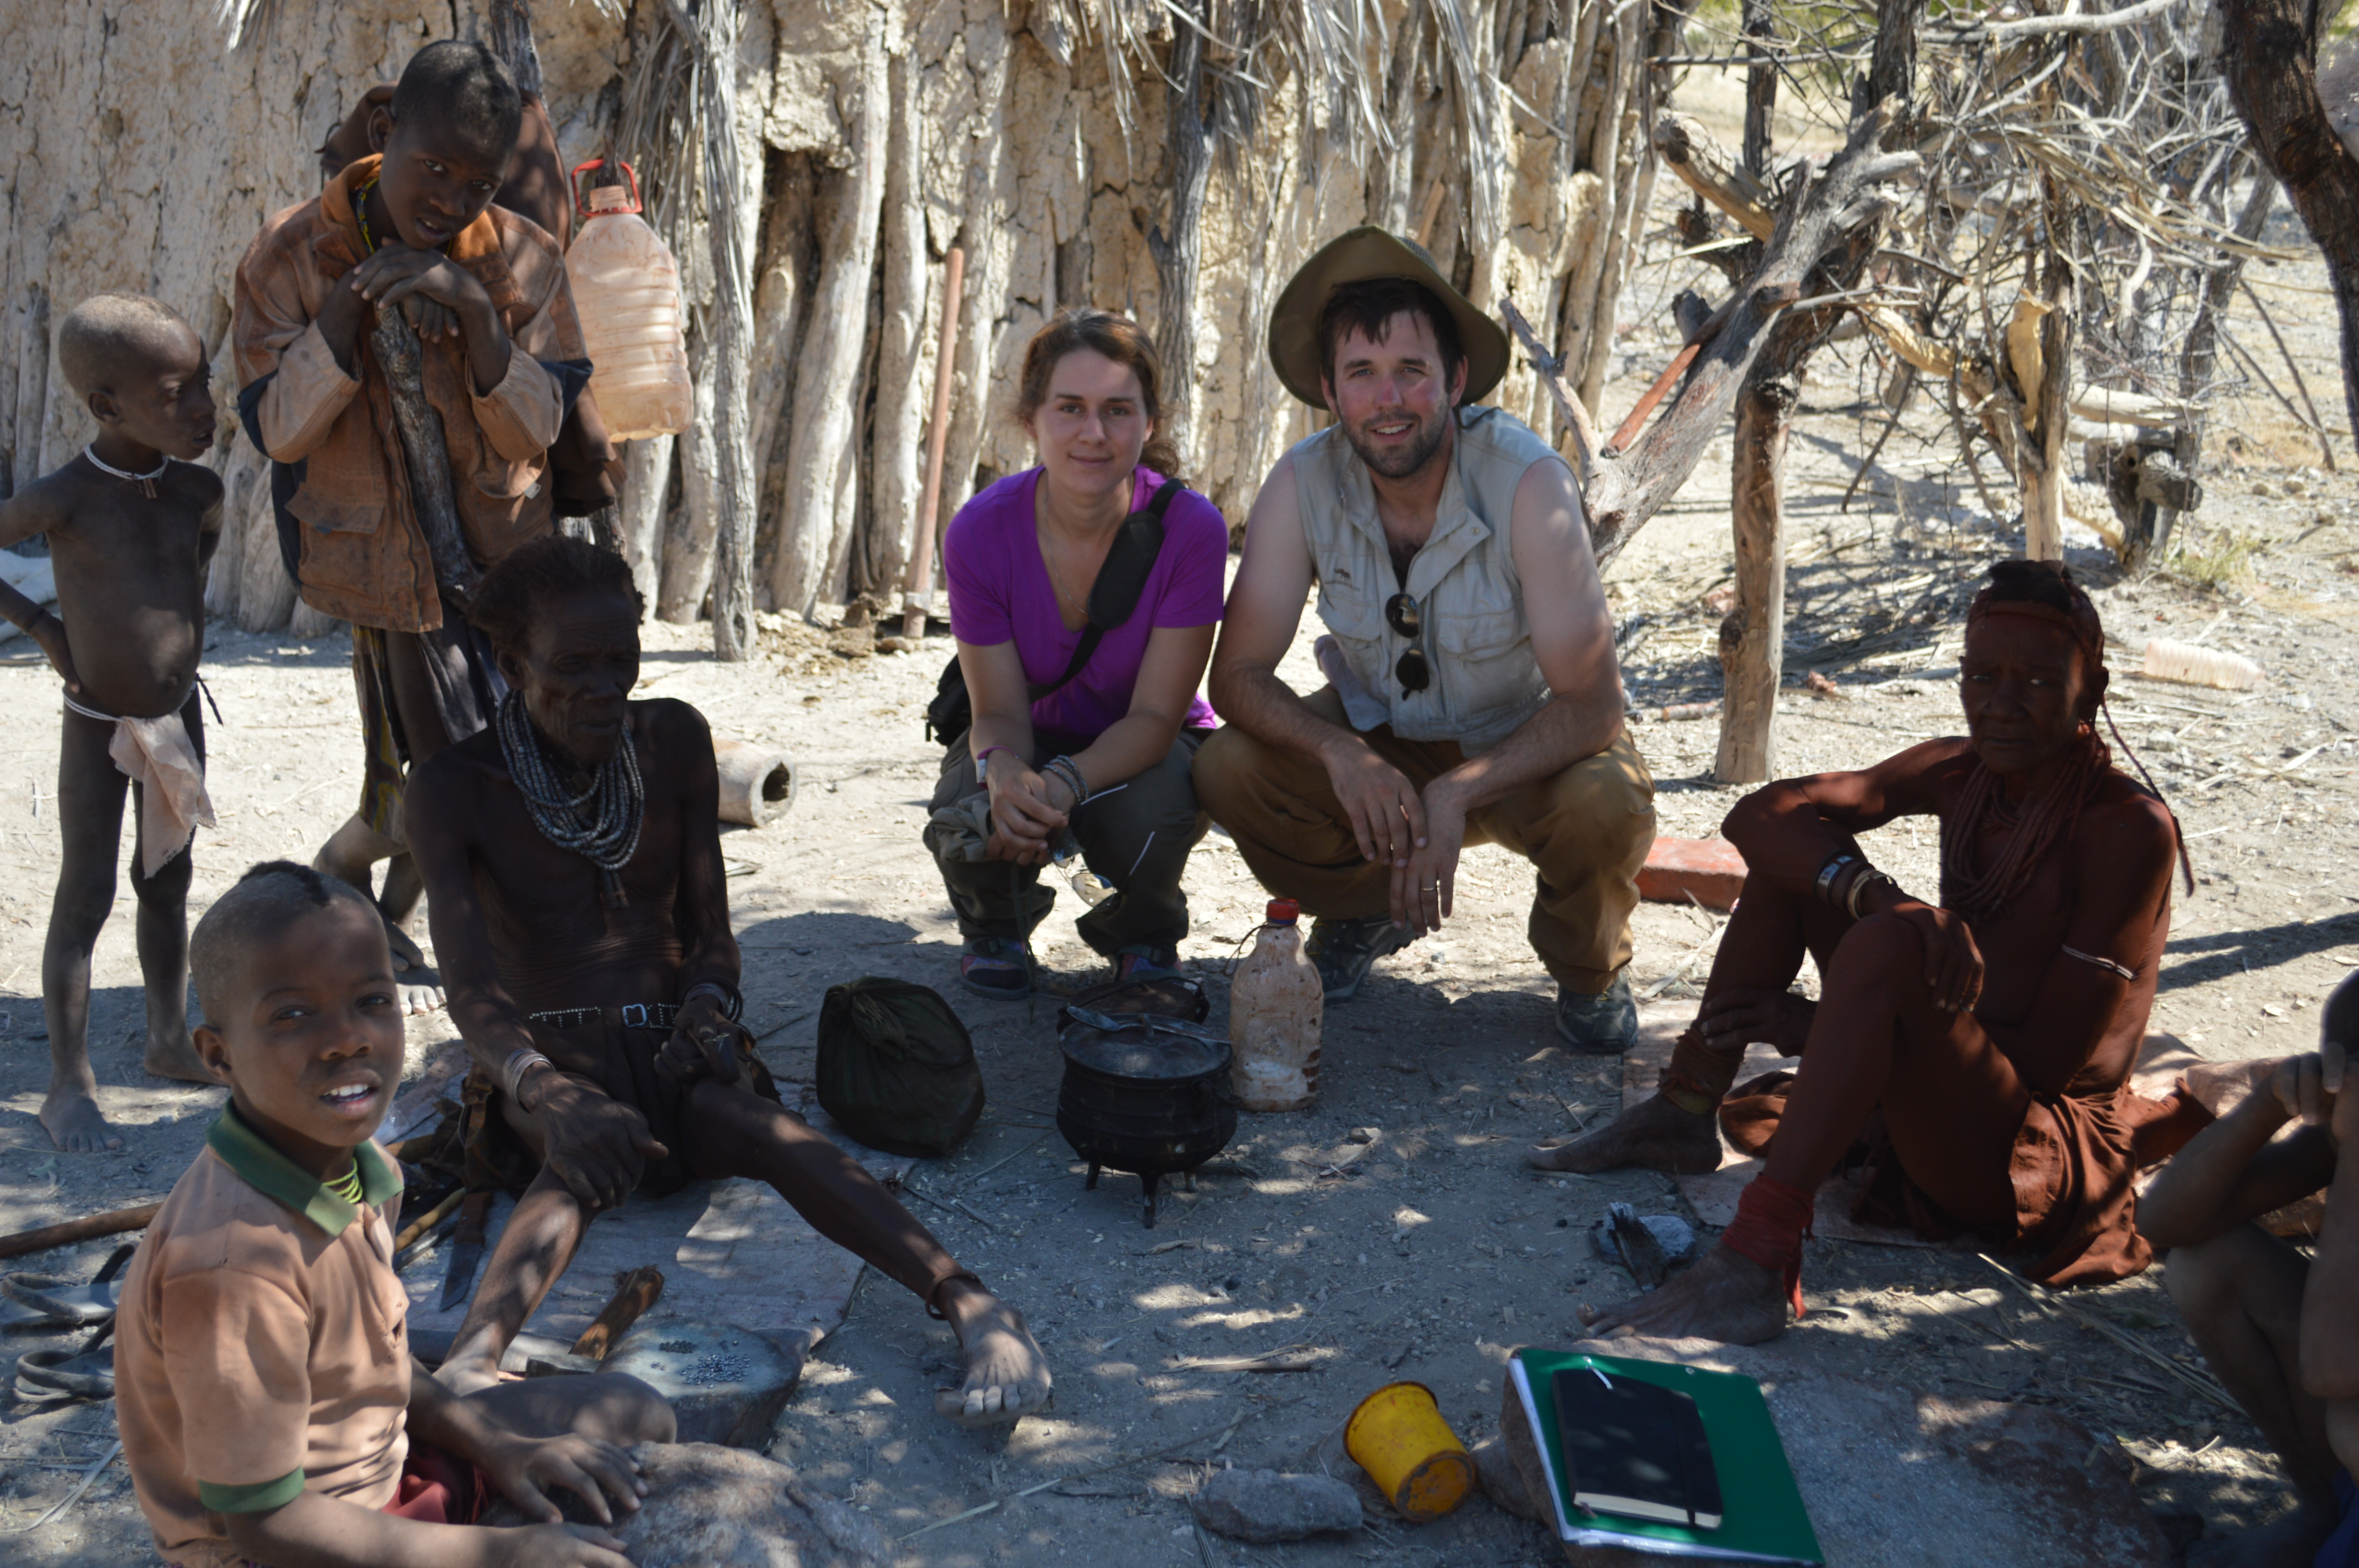
\includegraphics[width= .9\textwidth]{fieldwork}\\
\end{column}
\end{columns}

\end{frame}

%------------------------------------------------
%------------------------------------------------

\section{Empirical test}

%------------------------------------------------
%------------------------------------------------

\begin{frame}
\frametitle{Data}
\begin{columns}[c] % The "c" option specifies centered vertical alignment while the "t" option is used for top vertical alignment

\column{.45\textwidth} % Left column and width
\textbf{Subset:}
\begin{itemize} 
\item Women
\item Complete reproductive, genealogical, and marital data
\item Living mothers
\end{itemize}
88 unique women (195 observations). 

\column{.5\textwidth} % Right column and width
\begin{figure}
\includegraphics[width=1\linewidth]{datacol}
\end{figure}

\end{columns}
\end{frame}

%------------------------------------------------

\begin{frame}

\frametitle{Variables}

\textbf{Dependent variable:} 
\begin{itemize}
	\item Coresidence with mother \\
		\emph{``1'' same household or ``0'' different households}
\end{itemize}

\textbf{Key independent variables:}
\begin{itemize}
	\item \# of children $<$ 3 years old (``young children'')
	\item \# of daughters age 6 to 15 (``babysitters'')
\end{itemize}

\textbf{Control variables:}
\begin{itemize}
	\item Age
	\item Marriage
\end{itemize}

\vspace{0.5cm}
\textbf{Random effect:} by-participant random intercept


\end{frame}

%------------------------------------------------

\begin{frame}
\frametitle{Hypotheses}
\begin{enumerate}
\item \textbf{Women with young children are more likely to live with their mothers.}
\vspace{0.5cm}
\item \textbf{Women with babysitters are less likely to live with their mothers.}
\end{enumerate}
\end{frame}

%------------------------------------------------

\begin{frame}
\frametitle{H1: \\ Women with young children are more likely to live with their mothers}

DV = Coresidence with mother?;
\alert{$x_1 =$ \# young children}
\begin{equation*}
ln\left(\frac{\hat{p}}{(1 - \hat{p})}\right) = -0.73 \alert{ + 1.03x_{1}}
\end{equation*}

\begin{table}[h]
\caption {\textbf{Odds Ratio}}
  \centering
  \begin{tabular}{| l | r r r|} 
  	\hline
	\emph{IV} & Low & Est & Upp \\ \hline
	\# young children & \alert{1.5} & \alert{2.81} & \alert{5.24}\\	 \hline
	\multicolumn{4}{l}{ICC = .55}\\
  \end{tabular}
\end{table}
\end{frame}

%------------------------------------------------

\begin{frame}
\frametitle{H2: \\ Women with babysitters are less likely to live with their mothers}

DV = Coresidence with mother?;
$x_1 =$ \# young children; \alert{$x_2 =$ \# babysitters}
\begin{equation*}
ln\left(\frac{\hat{p}}{(1 - \hat{p})}\right) = -0.19 + 0.94x_{1} \alert{ - 0.69x_{2}}
\end{equation*}

\begin{table}[h]
\caption {\textbf{Odds Ratio}}
  \centering
  \begin{tabular}{| l | r r r|} 
  	\hline
	\emph{IV} & Low & Est & Upp \\ \hline
	\# young children & 1.35 & 2.56 & 4.86\\
	\# babysitters & \alert{0.32} & \alert{0.5} & \alert{0.79}\\	 \hline
	\multicolumn{4}{l}{ICC = .54}\\
  \end{tabular}
\end{table}
\end{frame}

%------------------------------------------------

\begin{frame}
\frametitle{Predicted prob. w/ age-specific means}
\begin{figure}
\includegraphics[width=0.6\linewidth]{nomarpred}
\end{figure}
\end{frame}

%------------------------------------------------

\begin{frame}
\frametitle{Predicted prob. w/ age-specific means}
\begin{figure}
\includegraphics[width=0.6\linewidth]{nomar}
\end{figure}
\end{frame}


%------------------------------------------------

\begin{frame}
\frametitle{Controlling for age}

DV = Coresidence with mother?;
$x_1 =$ \# young children; $x_2 =$ \# babysitters; \alert{$x_3 =$ age}
\begin{equation*}
ln\left(\frac{\hat{p}}{(1 - \hat{p})}\right) = 1.27 + 0.75x_{1} - 0.53x_{2} \alert{- 0.05x_{3}}
\end{equation*}

\begin{table}[h]
\caption {\textbf{Odds Ratio}}
  \centering
  \begin{tabular}{| l | r r r|} 
  	\hline
	\emph{IV} & Low & Est & Upp \\ \hline
	\# young children & 1.09 & 2.11 & 4.09\\
	\# babysitters & 0.36 & 0.59 & 0.95\\
	age & \alert{0.89} & \alert{0.95} & \alert{1.02}\\	 \hline
	\multicolumn{4}{l}{ICC = .48}\\
  \end{tabular}
\end{table}
\end{frame}

%------------------------------------------------

\begin{frame}
\frametitle{Importance of marriage}
\begin{figure}
\includegraphics[width=0.6\linewidth]{obs_crmom}
\end{figure}
\end{frame}

%------------------------------------------------

\begin{frame}
\frametitle{Controlling for marriage}

DV = Coresidence with mother?;
$x_1 =$ \# young children; $x_2 =$ \# babysitters; $x_3 =$ age; \alert{$x_4 =$ married?} 
\begin{equation*}
ln\left(\frac{\hat{p}}{(1 - \hat{p})}\right) = 2.26 + 0.94x_{1} - 0.68x_{2} - 0.03x_{3} \alert{- 2.81x_{4}}
\end{equation*}

\begin{table}[h]
\caption {\textbf{Odds Ratio}}
  \centering
  \begin{tabular}{| l | r r r|} 
  	\hline
	\emph{IV} & Low & Est & Upp \\ \hline
	\# young children & 1.22& 2.56 & 5.36\\
	\# babysitters & 0.30 & 0.51 & 0.86\\
	age & 0.97 & 0.9 & 1.05\\
	married? & \alert{0.02} & \alert{0.06} & \alert{0.16}\\\hline
	\multicolumn{4}{l}{ICC = .47}\\ 
  \end{tabular}
\end{table}
\end{frame}

%------------------------------------------------

%\begin{frame}
%\frametitle{Explaining delayed dispersal}
%\begin{figure}
%\includegraphics[width=0.6\linewidth]{withmar}
%\end{figure}
%\end{frame}

%------------------------------------------------

\begin{frame}
\frametitle{Additional analyses}
\begin{itemize}
\item Same patterns observed at household and village levels
\vspace{0.5cm}
\item Babysitter effect is unique to girls
\vspace{0.5cm}
\item Young women delay marriage until they have a babysitter
\vspace{0.5cm}
\item Residence effects of sisters, brothers, and fathers
\end{itemize}
\end{frame}

%------------------------------------------------

%\begin{frame}
%\frametitle{Discussion}
%\begin{itemize}
%\item Women often move away after marriage (Spousal bargaining or new opportunity?)
%\vspace{0.5cm}
%\item Evolutionary implications?
%\vspace{0.5cm}
%\item Impact of heritable wealth?
%\end{itemize}
%\end{frame}

%------------------------------------------------

\begin{frame}
\frametitle{Conclusion}
Residence patterns among foragers are highly flexible. \\
\vspace{0.5cm}
Interesting pattern within flexibility is delayed female dispersal. \\
\vspace{0.5cm}
Working from perspective of woman mapping onto childcare assistance helps explain pattern:
\begin{itemize}
\item Need maternal grandmother early
\item Early-born daughters free women to move away
\end{itemize}
\end{frame}

%------------------------------------------------

\begin{frame}
\frametitle{Acknowledgments}

\begin{columns}
\begin{column}{.8\textwidth}
\centering
\includegraphics[width= .6\textwidth]{chelsea}\\
\includegraphics[width= .6\textwidth]{steve}
\end{column}

\begin{column}{.2\textwidth}
\includegraphics[width= .8\textwidth]{NSF_logo}\\
\includegraphics[width= .8\textwidth]{WG_logo}
\end{column}
\end{columns}

\end{frame}

%------------------------------------------------

\begin{frame}
\Huge{\centerline{The End}}
\end{frame}

%----------------------------------------------------------------------------------------

\end{document}